\chapter{Introducción a los algoritmos genéticos y meméticos} \label{chapter:1}
 Las metaheurísticas, en su definición original, son métodos para calcular soluciones para problemas complejos que orquestan la interacción entre procedimientos de mejora local y estrategias de alto nivel, que permiten escapar de mínimos locales y una búsqueda robusta del espacio de soluciones \cite{metah-hb}. Sin embargo, las metaheurísticas, al contrario que los métodos de optimización clásicos, no siempre consiguen la solución óptima. Pese a esto, las metaheurísitcas son útiles para problemas cuyo conjunto de soluciones no sea computacionalmente tratable. Para conocer más sobre este tipo de problemas, se debe consultar el anexo \ref{anexoCC}.\par
 
En este primer capítulo se presentarán los principales resultados que rigen los algoritmos a tratar, además de explicar su funcionamiento en profundidad. En general, los algoritmos genéticos y meméticos pertenecen a un grupo más grande de algoritmos denominados algoritmos evolutivos.
\definition {Los algoritmos evolutivos son un tipo de algoritmo que se basan en principios de evolución biológica: estos principios incluyen la recombinación, la mutación y la selección \cite{evolutionary}.}\\

Estos algoritmos consiguen buenas soluciones por lo general, al no realizar ninguna suposición sobre el paisaje adaptativo. En las siguientes secciones se explicarán dos familias de este tipo de algoritmo: los algoritmos genéticos y los algoritmos meméticos. En primer lugar, veremos los conceptos básicos a tratar para entenderlos.
\section{Conceptos básicos}\label{intro:intro}
\subsection{Algoritmos y optimización combinatoria}
En primer lugar veamos conceptos básicos necesarios para definir los distintos métodos de solución que se tratarán posteriormente. Durante esta sección se utilizarán los conceptos introducidos por el capítulo 6 en \cite{metah-hb}.\\

\begin{definition}
    {Un \textit{algoritmo} es una secuencia de pasos lógicos o matemáticos que permiten resolver un problema computacional.}
\end{definition}
Un problema computacional $\mathcal{P}$ denomina una clase de tareas algorítmicamente realizables. Para cada problema $\mathcal{P}$ se definen las instancias de entrada del problema como el conjunto $I_\mathcal{P}$. Para cada $x\in I_\mathcal{P}$ existe un conjunto de \textbf{soluciones factibles} o aceptables denominado $\mathscr{S}(x)$ (el cual simplificaremos a $\mathscr{S}$ en el caso en el que no exista confusión).
\begin{definition}
    $\mathcal{X}$ es un \textit{conjunto de soluciones} del problema computacional $\mathcal{P}$ podemos definir la siguiente función que actúa sobre cada instancia $x\in I_\pcal$,
\[
\begin{tikzpicture}[node distance=1mm]
    \node (functionName) at (0, 0) {$c$:};
    \node[right = of functionName] (domain) {$I_\pcal$};
    \node[below = 2mm of domain] (element) {$x$};
    \node[right = 1cm of domain] (codomain) {$\mathcal{X}$};
    \node at (element-|codomain) (image) {$c(x)=y$,};
    \draw[-to] (domain) -- (codomain);
    \draw[|-to] (element) -- (image);
\end{tikzpicture}
\]
donde $c$ es la función definida por el algoritmo elegido. Los elementos $y\in\mathcal{X}$ satisfacen las condiciones del problema. El conjunto $\xcal$ se suele denominar soluciones dadas (ya que son las soluciones obtenidas a partir del algoritmo).
\end{definition} 

Un problema computacional se puede clasificar en los siguientes tipos según las metas que se plantea:
\begin{itemize}
    \item Búsqueda de todas las soluciones de $\scal$.
    \item Conteo del número de soluciones de $\scal$.
    \item Determinar si existen soluciones en $\scal$.
    \item Buscar una solución en $\scal$ tal que maximice o minimice una cierta función $m$, denominada función objetivo. Se denominan \textbf{problemas de optimización matemática} y este es el tipo de problemas que se tratarán en el resto del trabajo. 
\end{itemize}

\begin{definition}
    Se dice que una solución $y\in\xcal$ es \textit{factible} si es aceptable para una instancia $x\in I_\pcal$ del problema computacional $\pcal$. Es decir, si dado el resultado $y$ se tiene que $y \in \scal(x)$. De manera similar, se dice que un algoritmo resuelve un problema si la condición anterior se cumple para toda instancia $x\in I_\pcal$.
\end{definition}

Debido a que esta definición puede resultar poco útil en la práctica, al ser muy general, se pueden definir un tipo más específico de problemas computacionales, los \textbf{problemas de optimización combinatoria}.

\begin{definition}
    Los \textit{problemas de optimización combinatoria} son un conjunto de los problemas computacionales que para cada $x\in I_\pcal$ satisfacen las siguientes condiciones:
\begin{enumerate}
    \item $|\scal(x)|<\infty$.
    \item $\forall y \in \scal(x),\, \exists m(x,y)$, obtenido a partir de la función objetivo $m:I_\pcal\times\scal\longrightarrow A$, siendo $A$ el conjunto donde toma valores la función objetivo (por lo general $A=\mathbb{R}$).
    \item Existe $\prec_\pcal$ un orden parcial definido sobre los valores obtenidos a partir de la función objetivo $m$. En particular, si $A=\mathbb{R}$ entonces el orden parcial es el orden usual de $\mathbb{R}$.
\end{enumerate}
\end{definition} 

De esta manera, tendremos que una solución $\hat{y}\in\scal(x)$ es solución de la instancia $x\in I_\pcal$ del problema de optimización combinatoria $\pcal$ si y sólo si $\forall y \in \scal(x),\, \hat{y}\prec_\pcal y$.\\

En el caso habitual en el que $A=\mathbb{R}$, se tendrá un problema de minimización si buscamos $\hat{y}\in\scal(x)\text{, tal que }\hat{y}\leq y, \,\forall y \in \scal(x)$; y uno de maximización si buscamos $\hat{y}\in\scal(x)\text{, t.q. }\hat{y}\geq y, \,\forall y \in \scal(x)$. Sin embargo, estos problemas pueden tratarse de manera equivalente, ya que cualquier problema de maximización puede transformarse en uno de minimización y viceversa.\\

A partir de este momento, los siguientes conceptos que se introducirán en la sección serán específicos de los problemas de optimización combinatoria.

% Para hacer funciones
%\function{f}{A}{x}{X}{y}
\subsection{Espacios de búsqueda}
Una vez definido el concepto de la optimización combinatoria, es decir, la obtención de al menos una solución óptima de una instancia $x\in I_\pcal$ del problema computacional $\pcal$, veamos el concepto de los \textbf{espacios de búsqueda}. Para conseguir hallar el óptimo, $\hat{y}$, se utilizarán distintos \textbf{algoritmos de búsqueda}, donde se encuentran los algoritmos evolutivos. Sin embargo, para definir estos algoritmos será necesario especificar los conceptos de espacio de búsqueda, \textbf{relación de vecindad} y \textbf{función guía} \cite{metah-hb}. Comencemos por el primero.

\begin{definition}\label{def:esp-busq}
    Dada $x\in I_\pcal$ una instancia del problema $\pcal$, se define el \textit{espacio de búsqued}a como el conjunto $\mathcal{S}_\pcal(x)$ (aunque se podrá escribir como $\mathcal{S}$ en el caso de que no haya equivocación) tal que se cumplen las siguientes propiedades:

\begin{itemize}
    \item Cada elemento del espacio de búsqueda $s\in\mathcal{S}_\pcal(x)$ representa una solución de $\xcal$. Es importante que $s\in \xcal$, es decir, $s$ representa una solución dada, tanto si es factible como si no.
    \item Al menos un elemento $s\in\mathcal{S}_\pcal(x)$ representa a un elemento óptimo $\hat{y}\in\scal$.
\end{itemize}
\end{definition} 

Cada elemento $s\in\mathcal{S}_\pcal(x)$ se denomina \textbf{configuración} y se relaciona con un elemento de $\xcal$ mediante una \textbf{función de crecimiento} $g$ tal que:\[
\function{g}{\mathcal{S}}{s}{\xcal}{y.}
\]

Como trabajamos con $\xcal$ y no con $\scal$ directamente, los algoritmos de búsqueda deben estar preparados para poder lidiar con soluciones infactibles. En caso de que el algoritmo cumpla las condiciones de la Definición \ref{def:esp-busq} y sepa resolver conflictos con las soluciones infactibles se dice que tenemos una \textbf{formulación válida}.\\

Para los algoritmos evolutivos, el espacio de búsqueda $\mathcal{S}$ se denominará \textbf{genotipo} y el conjunto de soluciones dadas $\xcal$ se denominará \textbf{fenotipo}, de manera que la función $g$ definida anteriormente será la función de crecimiento. De esta manera, el espacio de búsqueda ofrece una base sobre la que se formularán los distintos algoritmos de búsqueda. Las relaciones entre las posibles configuraciones de un espacio de búsqueda se relacionan mediante una relación de vecindad.

\begin{definition}
    Una \textit{relación de vecindad} se define como una función $\mathcal{N}:\mathcal{S}\rightarrow 2^\mathcal{S}$, tal que asigna a cada elemento $s\in\mathcal{S}$ un conjunto $\mathcal{N}(s)$ de configuraciones vecinas de $s$.
\end{definition}

El vecindario, claramente depende de la instancia $x\in I_\pcal$, es decir: $\mathcal{N}(s)\equiv\mathcal{N}_\pcal(s,x)$. Un concepto muy importante de los vecindarios es que no se suelen definir todos los elementos de manera explícita, sino que se define como un conjunto de movimientos que permiten cambiar hacia otra configuración.

\begin{definition}
    Un \textit{movimiento} de un vecindario es una modificación local de una configuración $s\in \mathcal{S}$ de tal manera que se consiga otra distinta $s'\in\mathcal{N}(s)$ realizando una modificación total o parcial de la misma. La localidad indica que la modificación se produce solo en una solución para obtener otra solución vecina. En el contexto de los algoritmos evolutivos este proceso se denomina \textbf{mutación}.
\end{definition}

La idea de localidad es la que rige los algoritmos de búsqueda locales, los cuales se presentarán posteriormente. Dentro de los espacios de búsqueda falta por tratar la función de guía:

\begin{definition}
    Dado un conjunto $\mathscr{F}$ (normalmente se toma $\mathscr{F}\equiv\mathbb{R}$) con un orden parcial $\prec_\mathscr{F}$ (normalmente $\prec_\mathscr{F}\equiv <$) cuyos elementos se denominan valores de aptitud, la \textit{función de guía} es una función:
    \[\function{F_g}{\mathcal{S}}{s}{\mathscr{F}}{q,}\] donde $q$ valora la calidad de la solución. Esta función tiene la labor de controlar el comportamiento del algoritmo de búsqueda del espacio de soluciones.
\end{definition}

En los problemas de optimización la función de guía $F_g$ está directamente relacionada con la función objetivo $m$, y en casi todos los casos se tendrá que $F_g\equiv m$. Es decir, la función que guía el algoritmo de optimización será la función objetivo. Sin embargo, pueden existir casos donde esto no sea así, y que utilizar de manera directa la función objetivo sea contraproducente. Este es el caso en los problemas de optimización con restricciones, es decir, aquellos problemas donde $\scal \subset \xcal$. Como la función de crecimiento establece una relación entre $\mathcal{S}$ y $\xcal$, se pueden dar soluciones no válidas. Por consecuencia, la función de guía tiene que tener en cuenta las soluciones infactibles. De esta manera, puede definirse una función de guía que sea una suma con pesos de la función objetivo y la distancia a la factibilidad, donde se le da más importancia a que las soluciones sean factibles a que minimicen la función objetivo.

\begin{definition}
    La combinación del espacio de búsqueda, la relación de vecinidad y la función de guía con una instancia de un problema, induce un \textit{paisaje de adecuación}. Es decir, un grafo con pesos donde cada vértice denota una configuración $s\in\mathcal{S}$ y los arcos denotan las diferencias en la función de guía para cada configuración.
\end{definition}
Utilizando este concepto, el proceso del algoritmo de búsqueda puede verse como la navegación del paisaje utilizando la información de la función de guía. Podemos ver un ejemplo de paisaje de adecuación en la Figura \ref{fig:fit-lands}.
\begin{figure}[ht]
    \hspace{5.5cm}
    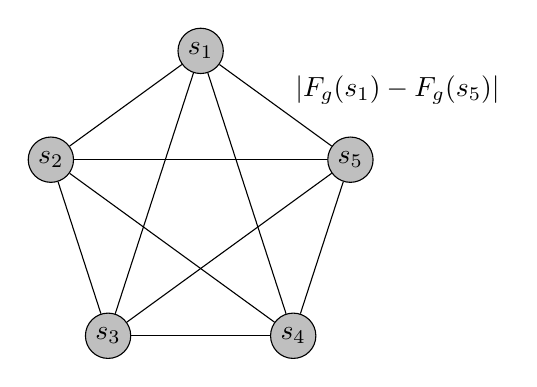
\begin{tikzpicture}
        
        % Define the number of nodes
        \def\n{5}  % Change this for more nodes
        \def\radius{2cm}
        
        % Place nodes in a circular pattern
        \foreach \i in {1,...,\n} {
            \node[draw,circle, fill=gray!50, inner sep=2pt, minimum size=15pt] (s\i) at ({(360/\n * (\i-1))+90}:\radius) {$s_{\i}$};
        }
        
        % Connect every node to every other node
        \foreach \i in {1,...,\n} {
            \foreach \j in {1,...,\n} {
                \ifnum\i<\j
                    \draw (s\i) -- (s\j);
                \fi
            }
        }
        \node (node) at (2.5,1.5) {$|F_g(s_1)-F_g(s_5)|$};
    \end{tikzpicture}
    \caption{Ejemplo de paisaje de adecuación. El peso de la arista depende de $F_g$.}
    \label{fig:fit-lands}
\end{figure}

\subsection{Búsqueda local y búsqueda basada en poblaciones}
Los conceptos anteriores inducen de manera directa el concepto de búsqueda local.

\begin{definition}
    Un \textit{algoritmo de búsqueda local} es un algoritmo que comienza en una configuración $s_0\in\mathcal{S}$ y busca una solución moviéndose en el paisaje de adecuación a configuraciones mejores basadas en el orden parcial $\prec_\mathscr{F}$.
\end{definition}

La exploración del paisaje se realiza por iteraciones y el algoritmo finaliza cuando se haya cumplido un criterio de parada. El criterio de parada suele ser un número máximo de iteraciones, no haber conseguido mejoras en un número $j$ de iteraciones o la utilización de mecanismos que estimen la probabilidad de haber encontrado un óptimo local.\\

En el contexto de los algoritmos evolutivos, los movimientos realizados se denominan \textbf{mutaciones} y dependen de las características del problema. Sin embargo, el algoritmo se encuentra en una única configuración en cada momento. Si aumentamos el número de configuraciones nos encontramos ante un tipo de algoritmos basados en poblaciones.

\begin{definition}
    Los \textit{algoritmos basados en poblaciones} de $k\in\mathbb{N},\,k>2$ individuos son un tipo de algoritmo que comienza en un conjunto de configuraciones $S=\{s_0^0,s_0^1,\ldots,s_0^{k-1}\},\, s_0^j\in\mathcal{S}$, llamado población y explora el, ahora hipergrafo, del paisaje de adecuación. Es decir, cada individuo explora de manera independiente su vecindario.
\end{definition}

Cada uno de los vértices del hipergrafo está formado por el conjunto de las configuraciones que toma cada individuo de la población. Cada individuo intercambia la configuración en cada paso de la exploración basado en un método de \textbf{recombinación}. Este proceso es una evolución a poblaciones del proceso de mutación.

\begin{definition}\label{def:recombinacion}
    La \textit{recombinación} es un proceso a partir del cual un conjunto $S_{pad}$ formado por $n$ configuraciones (padres), se utiliza para crear un subconjunto $S_{des}\in\scal$ de $m$ configuraciones (descendientes), donde $n+m=k$. 
\end{definition}

Existen diversos métodos para realizar la recombinación. Estos métodos se denominan \textbf{operadores de recombinación} y existen múltiples tipos con distintas propiedades, que permiten que los operadores funcionen de manera independiente a la representación del problema \cite{memetic}. Estas propiedades son las siguientes:
\begin{itemize}
    \bditem{Respeto}: Un operador se denomina respetuoso en caso de que mantenga aquellos elementos comunes dentro de los padres al generar los descendientes.
    \bditem{Surtido}: Se dice que un operador realiza un buen surtido si puede generar descendientes que contengan cualquier combinación compatible con los padres.
    \bditem{Transmisión}: Se dice que un operador es transmisible en el caso de que las características de la descendencia provengan de alguno de los padres, es decir, un operador es transmisible en el caso de que genere descendencia sin añadir nueva información. Esta nueva información será añadida en el proceso de mutación.
\end{itemize}

Un tipo importante de recombinación es la denominada \textbf{cruce}.

\begin{definition}\label{def:cruce}
    El \textit{cruce} es un tipo de operador de recombinación donde la única entrada es el conjunto $S_{pad}$ y la complejidad computacional de ser aplicado es menor que $\mathcal{O}(N\log N)$, donde $N$ representa el tamaño de la entrada del problema.
\end{definition}

Este tipo de operador es la base del primer algoritmo que estudiaremos, el algoritmo genético.

\section{Algoritmos genéticos}\label{intro:geneticos}
De manera similar a la Sección \ref{intro:intro}, este capítulo se basará en el libro \cite{metah-hb}, específicamente el capítulo 5 que explica los algoritmos genéticos. En primer lugar, haremos una introducción histórica a los algoritmos genéticos, posteriormente se relacionarán los conceptos tratados en la sección anterior con los algoritmos genéticos, se dará un esquema del algoritmo y se explicará su funcionamiento.
\subsection{Historia}
El término de algoritmo genético (GA) es definido por John Holland a mediados de la década de los 70 del siglo XX en \cite{holland_ga}, donde se introducían conceptos más genéricos que aquellos que se utilizan en los GA actualmente. Sin embargo, el concepto de estrategias evolutivas o programación evolutiva ya existía desde los años 60 \cite{rechenberg-1973,evolutionary-programming}. La principal diferencia de los GA con respecto a los anteriores algoritmos evolutivos es el concepto de recombinación, tratado en la Definición \ref{def:recombinacion}. Los anteriores algoritmos utilizaban únicamente la idea de las mutaciones, por lo que se pueden ver estos algoritmos como búsquedas locales.\\

A lo largo de las siguientes décadas, distintos alumnos de Holland desarrollaron los GA, investigando sus características y capacidades en el mundo de la optimización, lo cual no era el papel principal descrito en \cite{holland_ga}. Este interés en el mundo de la optimización tomó una gran importancia a partir del libro \cite{goldberg-ga}, que produjo que aumentase el desarrollo de la teoría y los usos de los GA. Debido a los resultado exitosos obtenidos por los investigadores en metaheurísticas, los algoritmos genéticos tomaron mucha importancia en la década de los 90. En los siguientes años, se introdujeron mejoras sobre ellos y en la actualidad tienen mucha importancia para la resolución de problemas complicados. Veamos el funcionamiento de estos algoritmos.\\

\subsection{Conceptos básicos}
Los conceptos principales de los algoritmos genéticos vienen dados por aquellos tratados en la Sección \ref{intro:intro}, pero en esta sección se explicará como se ajustan las ideas a los algoritmos genéticos.\\

En primer lugar, cabe destacar cual es el problema de optimización que un algoritmo genético trata de resolver:

\begin{definition}
    Dado el conjunto $\xcal$ que contiene las soluciones del problema computacional, también conocidas como variables de decisión, y una función objetivo
    $$m:\xcal\rightarrow\mathbb{R},$$
    el problema de optimización que buscan resolver los algoritmos genéticos es la obtención del elemento $x\in\xcal$ que minimice la función $m$, es decir:
    \begin{equation}\label{eq:def_min}
        \arg\min_{x\in\xcal}m(x).
    \end{equation}
\end{definition}

Es importante resaltar que los algoritmos genéticos también pueden resolver problemas de maximización. Estos problemas son intercambiables, ya que un problema de maximización puede verse como una minimización de la función objetivo $-m$.\\

Como se indicaba en la Sección \ref{intro:intro}, en este tipo de algoritmos no se utiliza directamente el conjunto $\xcal$ (fenotipo), sino que se trabaja con un conjunto de configuraciones denominado espacio de búsqueda (genotipo), definido como el conjunto $\mathcal{S}$. Específicamente, trabajaremos con un conjunto $\mathscr{A}$ denominado \textbf{alfabeto}, formado por distintos signos (pueden ser símbolos binarios, todos los números posibles, letras y símbolos\ldots). Para trabajar con algoritmos genéticos utilizaremos el conjunto $\mathcal{S}=\mathscr{A}^l$, que representa aquellas cadenas (o configuraciones) de símbolos del alfabeto $\mathscr{A}$ de longitud $l$. Para pasar del genotipo al fenotipo se utiliza una función de crecimiento:
\[
\function{g}{\mathcal{S}}{s}{\xcal}{x.}
\]
Es conveniente que la función de crecimiento sea una función biyectiva, de esta manera solo existirá una posible representación para cada solución y viceversa. Como este alfabeto es un espacio de búsqueda, se tiene que las configuraciones $s\in\mathcal{S}$ pueden no representar una solución válida en el espacio de soluciones $\xcal$, por lo que los algoritmos genéticos tendrán que lidiar con este problema, lo que puede verse en mayor profudidad en \cite{colin_ga}. 

\begin{notation}
    Se denomina \textit{gen} a cada uno de de los elementos de la cadena $s\in\mathcal{S}$ y \textit{alelo} a los posibles valores que pueden tomar los elementos de la cadena $s$. Además las cadenas se denominarán \textit{cromosomas}.
\end{notation}

Para simplificar el paso por la función de crecimiento podemos reescribir la Ecuación \ref{eq:def_min} utilizando una composición que sigue el siguiente esquema (suponiendo que la función $g$ es biyectiva):
\[
\begin{tikzpicture}[node distance=1mm]
    \node (domain) {$\mathscr{A}^l=\mathcal{S}$};
    \node[right = 1cm of domain] (codomain) {$\mathcal{X}$};
    \node[right = 1cm of codomain] (cocodomain) {$\mathbb{R}.$};
    
    \draw[-to] (domain) -- (codomain) node[midway,above] {$g$};
    \draw[-to] (codomain) -- (cocodomain) node[midway,above] {$m$};
    \draw[-to, out=150, in=30, looseness=1.2] (domain) .. controls (1.2, -1) and (2.8, -1) .. (cocodomain) node[midway,below] {$f$};
\end{tikzpicture}
\]
Es decir, la función a minimizar será $f(s)=m(g(s))$, y el nuevo problema vendrá definido por:
\begin{equation}\label{eq:def_comp}
    \arg\min_{s\in\mathcal{S}} f(s).
\end{equation}

Para resolver este problema los GA utilizan analogías biológicas. La cría selectiva de plantas y animales busca obtener descendencia con características positivas, estas características están definidas por la manera en la que se combinan los cromosomas de los padres. Pasando esto a un contexto matemático, en los GA se utiliza búsqueda por población en la cual la función de guía es directamente la función objetivo. Recordando la sección anterior, en una búsqueda por poblaciones, la búsqueda se realiza modificando las configuraciones mediante un proceso de recombinación, al cual se le añade un proceso de mutación para añadir información extra a la nueva población. Las configuraciones padres del proceso de recombinación serán elegidas utilizando una función de adecuación basada en la función objetivo $f$. Esta función trata de eliminar la negatividad de la función, es decir, la función de adecuación será $h(f(s))$, donde se tiene que $h:\mathbb{R}\rightarrow\mathbb{R}^+$.\\

Como se indica en la Sección \ref{intro:intro}, la recombinación es el paso más importante de los algoritmos genéticos y el uso de una población es aquello que los diferencia de las búsquedas locales. En particular, en los GA se utiliza el cruce como proceso de recombinación. Además, el uso de la mutación es clave para la utilización de los algoritmos genéticos para la resolución de problemas de optimización como el Problema \ref{eq:def_comp}, consiguiendo añadir nueva información a las soluciones que permite explorar otros vecindarios y salir de mínimos locales. De esta manera, podemos definir un esquema del funcionamiento de un algoritmo genético genérico, que debe adaptarse para resolver cualquier problema de optimización. Este esquema será mostrado como el pseudocódigo que se encuentra en el Algoritmo \ref{alg:genetico}.

\begin{algorithm}[!htb]
    \caption{Algoritmo genético}
    \label{alg:genetico}
    \begin{algorithmic}[1]
        \State \textbf{Inicialización:}
        \State Elección de una población inicial de cromosomas
        \State \textbf{Optimización:}
        \While {criterio de terminación no satisfecho}
            \Repeat 
                \If {se satisface la condición de cruce}
                    \State Selección de los padres
                    \State Selección de los parámetros de cruce
                    \State Realización del cruce
                \EndIf
                \If {se satisface la condición de mutación}
                    \State Selección de los puntos de mutación
                    \State Realización de la mutación
                \EndIf
                \State Evaluación de la adecuación de la descendencia
            \Until {se haya generado el número necesario de descendencia}
            \State Selección de una nueva población
        \EndWhile
    \end{algorithmic}
\end{algorithm}

\subsubsection{Selección de la población inicial}\label{intro:sel-inicial}
Antes de comenzar, será necesario la elección de una población inicial a partir de la cual se realizará la optimización. En primer lugar, es importante decidir el tamaño de la población. El tamaño de la población deberá ser un compromiso entre eficiencia y efectividad en la búsqueda. Existen varios métodos para realizar esta selección, y existe mucha literatura que busca obtener un valor óptimo o cercano al óptimo dependiendo de la longitud de cadena. Esto conduce a problemas, ya que los métodos teóricos encontrados definen un número de individuos $M$ exponencialmente creciente \cite{goldberg1985optimal,goldberg1988sizing}.\\

Sin embargo, en la práctica, los métodos utilizando un menor número de individuos obtienen buenos resultados, por lo que se realizaron investigaciones no sobre el número óptimo, sino sobre el número mínimo de individuos necesarios para realizar una búsqueda efectiva. En esencia, el número mínimo de individuos es aquel que permita definir una población a partir de la cual sea posible alcanzar cualquier punto del espacio de búsqueda mediante únicamente la operación de cruce. Esto puede parecer complicado, pero solo es necesario que exista un alelo distinto en cada uno de los elementos del cromosoma. De esta manera, el número de individuos de la población será elegido de manera en la que en caso de generar los cromosomas de manera aleatoria, la probabilidad de que en cada posición existan todos los posibles valores sea lo más cercana al $100\%$. Esta probabilidad es sencilla de calcular para alfabetos binarios:
$$P_2^*=(1-(\frac{1}{2})^{M-1})^l.$$

Sin embargo, al pasar a alfabetos de $q$ elementos la expresión se complica. En \cite{colin-pq} se calcula esta probabilidad, obteniendo la siguiente expresión:
$$P_q^*=\left(\frac{q!S(M,q)}{q^M}\right)^l,$$
donde la función $S(M,q)$ representa un número de Stirling de segunda especie, que representa la cantidad de maneras para particionar un conjunto de $M$ elementos en $q$ subconjuntos. Es difícil comprender este número de manera intuitiva, no obstante, en el mismo trabajo se explica como el mínimo crece de manera logarítmica con la longitud de la cadena, lo que es muy interesante en la práctica.\\

Finalmente, una vez decidido el valor del tamaño de la población $M$, se deberá realizar la selección de individuos para la población inicial. Esta selección será aleatoria, específicamente, se realizará muestreo sin remplazo, garantizando que no existan individuos repetidos en la población inicial. También pueden utilizarse otros métodos, que aunque también aleatorios suelen conseguir que se cubra un mayor espacio muestral. Otra ``mejora'' que se puede hacer es la adición a la población de alguna buena solución obtenida por otros métodos heurísticos o mediante algoritmos voraces. Mediante esta técnica se puede conseguir obtener mejores soluciones antes, aunque puede provocar una convergencia prematura y mayor posibilidad de caer en mínimos locales.

\subsubsection{Criterio de parada}\label{intro:sel-criterio}
Al contrario de los métodos de búsqueda locales, que finalizan al encontrar un mínimo local, los algoritmos genéticos son métodos estocásticos que pueden funcionar de manera indefinida. Por consiguiente, será necesario definir un criterio de parada para el algoritmo. Normalmente este criterio será una condición que pueda calcularse de manera sencilla, evitando así introducir complejidad en el algoritmo.\\

El criterio de parada más común es haber cumplido un cierto número de iteraciones o haber realizado un número máximo de evaluaciones de adecuación (en esencia estos criterios son equivalentes). Sin embargo, pueden definirse criterios más complejos, como que la diversidad de la población sea inferior a un límite predefinido o que la proporción de uno de los alelos de toda la población alcance un límite alto. Actualmente no existe ningún método teórico que ofrezca un criterio de parada absoluto u óptimo, por lo que se deberá elegir aquel que ofrezca mejores resultados dependiendo del problema, volviendo otra vez al compromiso entre efectividad en la búsqueda y eficiencia del algoritmo.

\subsection{Selección}
Como se veía en el Pseudocódigo \ref{alg:genetico}, el primer paso en el proceso de cruce de un algoritmo genético es la selección de los padres. Este procedimiento puede parecer un paso secundario en el cruce, no obstante, es un paso muy importante por lo que en la literatura suele ser tratado como un proceso principal en los algoritmos genéticos. La selección deberá estar guiada por la función de adecuación y existen diversos métodos para realizarla.
\subsubsection{Método de selección de la ruleta}
Este método es el original para la selección de padres para un GA y se basa en la idea de la utilización de una distribución de probabilidad donde la probabilidad de elegir cada cadena depende de la adecuación. Es decir, cuanto mayor sea la adecuación de la cadena, mayor es la región de probabilidad. Para la selección se utiliza un número aleatorio entre 0 y 1, y este número decide la cadena. La selección de la región a partir de un número aleatorio se puede realizar en un tiempo $\mathcal{O}(\log M)$. Sin embargo, este método añade mucha variabilidad estocástica y el número de veces que un cromosoma es elegido puede diferir mucho de su esperanza teórica. Un ejemplo de este tipo de selección puede verse en la Figura \ref{fig:RWS}.\\

Para evitar estos problemas, se utiliza en la práctica la selección universal estocástica (SUE) \cite{beranek-1987}. En vez de realizar una única selección para cada cromosoma de la población, se eligen de manera simultánea los valores de todos los cromosomas de la población. Este método utiliza muestreo sistemático, es decir, se toma un número aleatorio inicial y se eligen $M$ elementos con un paso dado. De esta manera, se consigue eliminar la varibilidad estocástica del método anterior haciendo que sí que se tomen los elementos con la esperanza deseada. Un ejemplo de este tipo de selección puede observarse en la Figura \ref{fig:SUE}.\\

El principal problema de este método es encontrar una función de adecuación $h$ correcta. No solo debe tenerse en cuenta que la función objetivo puede tomar tanto valores positivos como negativos, sino que la diferencia entre los valores de la función también es importante, implicando la necesidad de un reescalado. Por ello, existen otros métodos que buscan evitar estos problemas.
\begin{figure}[t]
    \centering
    \begin{subfigure}[b]{0.49\textwidth}
        \centering
        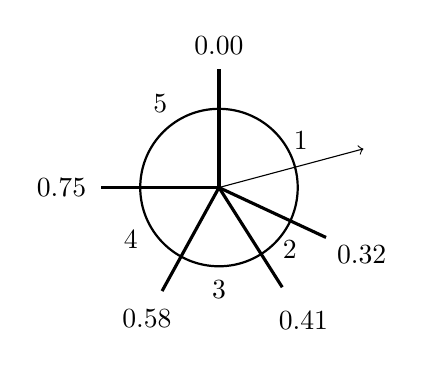
\begin{tikzpicture}
            \draw[thick] (0,0) circle (1);
            \node (nodo1) at (90:1.8) {$0.00$};
            \node (nodo2) at (-25:2) {$0.32$};
            \node (nodo3) at (-57.6:2) {$0.41$};
            \node (nodo4) at (-118.8:1.9) {$0.58$};
            \node (nodo5) at (180:2) {$0.75$};
            \node at (30:1.2) {$1$};
            \node at (-41.4:1.2) {$2$};
            \node at (-90:1.3) {$3$};
            \node at (-149.4:1.3) {$4$};
            \node at (125:1.3) {$5$};
            \draw[line width=0.4mm] (0,0) -- (90:1.5);
            \draw[line width=0.4mm] (0,0) -- (-25:1.5);
            \draw[line width=0.4mm] (0,0) -- (-57.6:1.5);
            \draw[line width=0.4mm] (0,0) -- (-118.8:1.5);
            \draw[line width=0.4mm] (0,0) -- (180:1.5);
            \draw[-to] (0,0) -- (15:1.9);
        \end{tikzpicture}
        \caption{Selección de ruleta, en un caso donde el número aleatorio es $0.29$, eligiendo la cadena 1.}
        \label{fig:RWS}
    \end{subfigure}
    \begin{subfigure}[b]{0.49\textwidth}
        \centering
        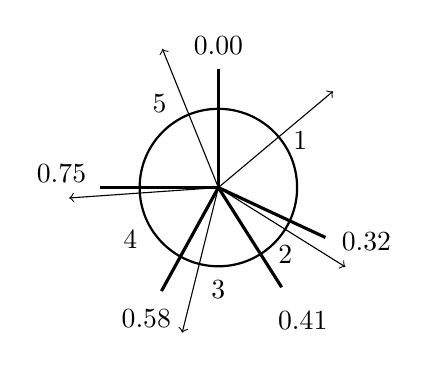
\begin{tikzpicture}
            \draw[thick] (0,0) circle (1);
            \node (nodo1) at (90:1.8) {$0.00$};
            \node (nodo2) at (-20:2) {$0.32$};
            \node (nodo3) at (-57.6:2) {$0.41$};
            \node (nodo4) at (-118.8:1.9) {$0.58$};
            \node (nodo5) at (175:2) {$0.75$};
            \node at (30:1.2) {$1$};
            \node at (-45:1.2) {$2$};
            \node at (-90:1.3) {$3$};
            \node at (-149.4:1.3) {$4$};
            \node at (125:1.3) {$5$};
            \draw[line width=0.4mm] (0,0) -- (90:1.5);
            \draw[line width=0.4mm] (0,0) -- (-25:1.5);
            \draw[line width=0.4mm] (0,0) -- (-57.6:1.5);
            \draw[line width=0.4mm] (0,0) -- (-118.8:1.5);
            \draw[line width=0.4mm] (0,0) -- (180:1.5);
            \draw[-to] (0,0) -- (40:1.9);
            \draw[-to] (0,0) -- (-32:1.9);
            \draw[-to] (0,0) -- (-104:1.9);
            \draw[-to] (0,0) -- (-176:1.9);
            \draw[-to] (0,0) -- (-248:1.9);
        \end{tikzpicture}
        \caption{Método SUE. Se toman 5 elementos equidistantes a partir del primer elemento generado aleatoriamente, $0.11$.}
        \label{fig:SUE}
    \end{subfigure}
    \caption{Distintas variaciones del método de selección por ruleta.}
    \label{fig:roulette-wheel}
\end{figure}


\subsubsection{Ranking}
El método de ranking se basa en la ordenación de los cromosomas por su adecuación (siendo la posición $M$ la que mayor adecuación tiene), eliminando los problemas de elección de la función $h$ tratados en el anterior método (sobre todo el problema del reescalado). El método más utilizado es el ranking lineal. Este ranking define la probabilidad de elegir el cromosoma en posición $k$ como:
$$P(k)=\alpha+\beta k,\quad P(k)\geq0,\quad \sum_{k=1}^M(\alpha+\beta k)=1,$$
donde $\alpha$ y $\beta$ son constantes y la segunda y tercera condición se tienen por ser $P$ una distribución de probabilidad. De esta manera podremos seleccionar la \textbf{presión de selección} de manera libre.

\begin{definition}
    La \textit{presión de selección}, $\phi$ se define como:
    $$\phi = \frac{P[seleccion\_mejor\_individuo]}{P[seleccion\_individuo\_medio]}.$$
\end{definition}
En el caso del ranking lineal, se tiene que la presión de selección vendrá dada por la siguiente expresión, a partir de la cual podemos obtener expresiones para los valores de $\alpha$ y $\beta$ de manera sencilla:
\begin{equation}\label{eq:alfabeta}
    \phi=\frac{\alpha+\beta M}{\alpha+\beta(M+1)/2}\implies \beta =\frac{2(\phi-1)}{M(M-1)},\,\alpha=\frac{2M-\phi(M+1)}{M(M-1)},
\end{equation}
donde suponemos que la población es de tamaño $M$, con $M$ un número impar mayor que $3$ (si es par, la expresión se modifica intercambiando $M+1$ por $M\geq2$).\\

Ahora, utilizando las expresiones anteriores tenemos el siguiente resultado que proporciona cotas inferior y superior para $\phi$.
\begin{proposition}
    En el caso de ranking lineal, el valor de la presión de selección, $\phi$, cumple las siguientes desigualdades:
    $$1\leq\phi\leq2.$$
    \begin{proof}
        En primer lugar, comprobamos que $P(k)=\alpha+\beta k$ (la probabilidad de elegir el cromosoma en la posición $k$), $k\in\{1,\ldots,M\}$ con $\alpha$ y $\beta$ como los dados por la Ecuación \ref{eq:alfabeta}, cumple $\sum_{k=1}^M(\alpha+\beta k)=1$. Aplicando la expresión de la suma de una progresión aritmética, se obtiene:        
        \begin{equation*}
            \begin{split}
                \sum_{k=1}^M(\alpha+\beta k)&=\alpha M+\beta\frac{M(M+1)}{2}=\frac{2M-\phi(M+1)}{M-1}+\frac{2(\phi-1)(M+1)}{2(M-1)}\\
                &=\frac{4M-2\phi M-2\phi+2\phi M+2\phi-2M-2}{2(M-1)}=\frac{2(M-1)}{2(M-1)}=1.
            \end{split}
        \end{equation*}

        En segundo lugar, se tiene que $\alpha+\beta k \geq 0,\,\forall k\in\{1,\ldots,M\}$.
        
        \noindent\textbullet\hspace{0.4cm}Notemos que si $\phi>2$, tomando $k=1$ y asumiendo que $M\geq2$, considerando el numerador de $\alpha+\beta\cdot 1=\alpha+\beta$, se obtiene:
        \begin{equation*}
            \begin{split}
                &2M-\phi(M+1)+2\phi -2=2M-\phi M-\phi+2\phi-2=M(2-\phi)+( \phi-2)=\\
                =&M(2-\phi)-(2-\phi)=(2-\phi)(M-1)<0
            \end{split}            
        \end{equation*}
        Como el denominador de $\alpha+\beta$ es siempre positivo, se tiene que $\alpha+\beta<0$. Por tanto, $\phi\leq2$.
         
        \noindent\textbullet\hspace{0.4cm} Si $k=M$ y tomando el numerador de $\alpha+\beta k$ se obtiene:
        $$2M-\phi(M+1)+2M\phi-2M=-\phi M-\phi+2M\phi=M\phi-\phi=\phi(M-1).$$
        Como $\alpha+\beta M\geq0$ se sigue que $\phi\geq0$.

        Falta comprobar que con $\phi\in[0,2]$ se cumple $\alpha+\beta k\geq0$ para los restantes valores de $k$. Distinguimos 2 casos:

        \begin{itemize}
            \item Si $k\geq(M+1)/2$, considerando el numerador de $\alpha+\beta k$:
            \[
            \underset{\overset{\scriptsize \rotatebox[origin=c]{90}{$\leq$}}{0}}{(2M - 2k)} 
            + \underset{\overset{\scriptsize \rotatebox[origin=c]{90}{$\leq$}}{0}}{\phi}\underset{\overset{\scriptsize \rotatebox[origin=c]{90}{$\leq$}}{0}}{(2k - M - 1)} 
            \geq 0, \quad \text{si } \phi \geq 0.
            \]
            \item Si $k<(M+1)/2$ ($M+1-2k>0$):
            $$2M-2k-\phi(M-1-2K)\geq 0 \iff \phi\leq\frac{2M-2k}{M+1-2k}.$$
            Distinguimos 2 subcasos:
            \begin{itemize}
                \item Si $k=1$: $$\frac{2M-2k}{M+1-2k}=\frac{2M-2}{M+1-2}=\frac{2(M-1)}{M-1}=2\geq\phi\in[0,2].$$
                \item Si $k>1$, $\frac{2M-2k}{M+1-2k}>2$, puesto que $2M-2k-2M-2+4k=2k-2>0$ y entonces:
                $$\frac{2M-2k}{M+2-2k}>2\geq\phi,\;\forall\phi\in[0,2].$$
            \end{itemize}
        \end{itemize}
        
        Por tanto, $\alpha+\beta k \geq 0,\;\forall k\in\{1,\ldots,M\}\implies \phi\in[0,2]$.
        
        Para terminar, descartamos los valores de $\phi\in[0,1)$ puesto que el objetivo es dar mayor probabilidad de selección a los mejores individuos, esto es, los más adecuados. Por tanto, finalmente $\phi\in[1,2]$ y la demonstración concluye.
    \end{proof}
\end{proposition}

Interpretando este resultado, cuanto más cerca se encuentre el valor de $\phi$ de 2, mayor será la probabilidad de que el cromosoma elegido sea el individuo más adecuado de la población, mientras que cuanto más cercano a 1, más probable será escoger individuos de manera aleatoria.\\

La principal ventaja que añade este método, además de ofrecer mayor control, es la facilidad de encontrar el individuo dado un número aleatorio $r\in[0,1]$. Para ello utilizaremos la función de distribución de probabilidad $F(k)=\sum_{k'=1}^k(\alpha+\beta k')$. Como esta función es una progresión aritmética, dado un número $r$, el valor $k$ que genera esta probabilidad vendrá dado por la ecuación de segundo grado:
$$\alpha k+\beta\frac{k(k+1)}{2}=r\implies k = \frac{-(2\alpha+\beta)\pm \sqrt{(2\alpha+\beta)^2+8\beta r}}{2\beta},$$
cuya solución puede ser obtenida en un tiempo constante. Aunque existen más tipos de ranking (por ejemplo el ranking exponencial \cite{exponential-ranking} o el algoritmo GENITOR \cite{genitor}), el ranking lineal es suficiente para la mayor parte de los problemas.
\subsubsection{Método de selección por torneo}
Este método está basado en la competición de un conjunto de $\tau$ cromosomas en un torneo binario donde en cada ronda avanza el cromosoma con mayor adecuación. El número $\tau$ de cromosomas elegido depende del problema y de la implementación, por ejemplo, si $\tau=2$, se tiene un método de selección de ranking lineal con $\phi=1$, y si $\tau=M$, se elige al cromosoma con mayor adecuación de toda la población.

\begin{figure}[t]
    \centering
    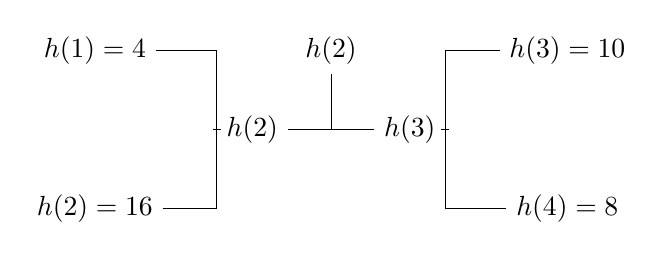
\begin{tikzpicture}
        \node (a) at (0,1) {$h(1) = 4$};
        \node (b) at (0,-1) {$h(2) = 16$};
        \node (ab) at (2,0) {$h(2)$};
        \node (winner) at (3,1) {$\boldsymbol{h(2)}$};
        \node (cd) at (4,0) {$h(3)$};
        \node (c) at (6,1) {$h(3) = 10$};
        \node (d) at (6,-1) {$h(4) = 8$};

        \draw (a) -| (ab.west);
        \draw (b) -| (ab.west);
        \draw (ab) -| (winner.south);
        \draw (c) -| (cd.east);
        \draw (d) -| (cd.east);
        \draw (cd) -| (winner.south);
        \draw (1.5,0) -- (1.6,0);
        \draw (4.5,0) -- (4.4,0);
    \end{tikzpicture}
    \caption{Ejemplo de una selección por torneo para $\tau=4$. El elemento seleccionado, al tener una mayor adecuación sería el cromosoma 2.}
    \label{fig:sel-torneo}
\end{figure}

Este método es muy sencillo de entender y una de las ventajas más grandes que tiene es que puede funcionar sin función objetivo explícita, ya que solo necesita comparar pares de cromosomas entre ellos, pudiendo utilizar un criterio ``subjetivo''. Un ejemplo de este método puede verse en la Figura \ref{fig:sel-torneo}. Sin embargo, los problemas de este método son similares a los de la selección por ruleta, ya que la elección de los participantes del torneo es aleatoria. Para disminuir esta aleatoriedad, se pueden utilizar métodos como el propuesto en \cite{tournament}. Como tenemos que extraer $\tau$ elementos $M$ veces, generamos $\tau$ permutaciones aleatorias de los números desde 1 hasta $M$. Estas permutaciones serán concatenadas en una cadena y se irán cogiendo los elementos de $\tau$ en $\tau$ elementos para participar en torneos sucesivos, de esta manera, habremos seleccionado $M$ cromosomas en torneos donde han participado todos los cromosomas de la anterior generación.

\subsection{Cruce}

En los algoritmos genéticos se utiliza un tipo de recombinación para generar los descendientes denominado cruce (véase Definición \ref{def:cruce}). Hay múltiples algoritmos para realizar el cruce para un algoritmo genético pero los más importantes son: cruce de $m$ puntos, cruce uniforme y cruce no lineal.\\

El \textbf{cruce de $m$ puntos} se basa en la selección de $m$ números aleatorios entre 1 y $l-1$ (sin repeticiones), siendo $l$ el número de alelos que forman cada cromosoma. Una vez elegidos los puntos de cruce, se genera la descendencia combinando los alelos de los padres entre esos puntos. En la Figura \ref{fig:2xcrossover}, podemos ver un ejemplo de este tipo de cruce, en específico un cruce de 2 puntos. El principal problema de este cruce es la adición de sesgo posicional y sesgo distribucional. Dependiendo del número de puntos de cruce estos dos sesgos aumentan, con diversos estudios apuntando a que el cruce de 8 puntos es el mejor.

% \begin{figure}
%     \centering
%     \begin{tikzpicture}.
%         \node at (0,0) {P1 $\rightarrow1\ 0\ 1\ 0\ 0\ 1\ 1$};
%         \node at (0,-1) {P2 $\rightarrow1\ 1\ 0\ 0\ 1\ 1\ 0$};
%         \node at (0.05,-0.5) {$\updownarrow$};
%         \node at (1.3,-0.5) {$\updownarrow$};
%         \node at (5,0) {H1 $\rightarrow1\ 0\ 0\ 0\ 1\ 1\ 1$};
%         \node at (5,-1) {H2 $\rightarrow1\ 1\ 1\ 0\ 0\ 1\ 0$};
%         \draw[-to] (2,-0.5) -- (3,-0.5);
%     \end{tikzpicture}
%     \caption{Ejemplo de cruce de 2 puntos (2 y 6) para un alfabeto binario. El hijo 1 tiene los dos primeros alelos y el último del padre 1, el resto del padre 2.}
%     \label{fig:2xcrossover}
% \end{figure}

\begin{figure}[t]
    \centering
    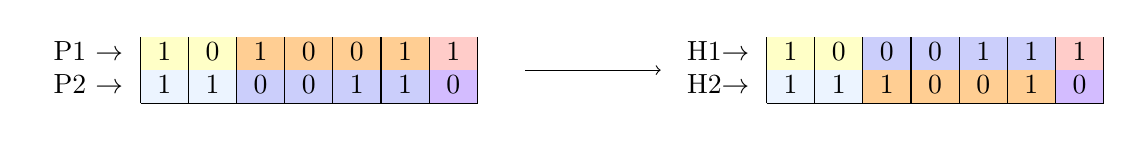
\begin{tikzpicture}
        \node (padres) at (0,0) {\begin{tabular}{l| >{\columncolor[HTML]{FFFFC7}}c |
            >{\columncolor[HTML]{FFFFC7}}c |
            >{\columncolor[HTML]{FFCE93}}c |
            >{\columncolor[HTML]{FFCE93}}c |
            >{\columncolor[HTML]{FFCE93}}c |
            >{\columncolor[HTML]{FFCE93}}c |
            >{\columncolor[HTML]{FFCCC9}}c |}
            \cline{2-8}
            P1 $\rightarrow$ & $1$ & $0$ & $1$ & $0$ & $0$ & $1$ & $1$ \\ \cline{2-8} 
            P2 $\rightarrow$ & \cellcolor[HTML]{ECF4FF}$1$ & \cellcolor[HTML]{ECF4FF}$1$ & \cellcolor[HTML]{CBCEFB}$0$ & \cellcolor[HTML]{CBCEFB}$0$ & \cellcolor[HTML]{CBCEFB}$1$ & \cellcolor[HTML]{CBCEFB}$1$ & \cellcolor[HTML]{D3BCFF}$0$ \\ \cline{2-8} 
            \end{tabular}};
        \node (hijos) at (8,0) {\begin{tabular}{l|
            >{\columncolor[HTML]{FFFFC7}}c |
            >{\columncolor[HTML]{FFFFC7}}c |
            >{\columncolor[HTML]{CBCEFB}}c |
            >{\columncolor[HTML]{CBCEFB}}c |
            >{\columncolor[HTML]{CBCEFB}}c |
            >{\columncolor[HTML]{CBCEFB}}c |
            >{\columncolor[HTML]{FFCCC9}}c |}
            \cline{2-8}
            H1$\rightarrow$ & $1$ & $0$ & $0$ & $0$ & $1$ & $1$ & $1$ \\ \cline{2-8} 
            H2$\rightarrow$ & \cellcolor[HTML]{ECF4FF}$1$ & \cellcolor[HTML]{ECF4FF}$1$ & \cellcolor[HTML]{FFCE93}$1$ & \cellcolor[HTML]{FFCE93}$0$ & \cellcolor[HTML]{FFCE93}$0$ & \cellcolor[HTML]{FFCE93}$1$ & \cellcolor[HTML]{D3BCFF}$0$ \\ \cline{2-8} 
        \end{tabular}};
        \draw[-to] (3.4,0) -- (hijos);
    \end{tikzpicture}
    \caption{Ejemplo de cruce de 2 puntos (2 y 6) para un alfabeto binario. El hijo 1 tiene los dos primeros alelos y el último del padre 1, el resto del padre 2.}
    \label{fig:2xcrossover}
\end{figure}

El segundo tipo importante de cruce es el \textbf{cruce uniforme}, este cruce es en esencia un cruce aleatorio. Este cruce se realiza utilizando una \textbf{máscara}.
\begin{definition}\label{def:mascara}
    Una \textit{máscara} es una cadena binaria de $l$ elementos que representa a qué padre pertenecen los alelos de un hijo. En el caso de que el valor del elemento $i$ de la máscara valga 1 el elemento pertenecerá al padre 1 y en el caso contrario al padre 2.
\end{definition}
En el cruce uniforme, las máscaras son generadas de manera estocástica mediante una distribución de Bernoulli. El parámetro $p$ de esta distribución no tiene por que ser $0.5$ y puede estar sesgada hacia alguno de los dos padres, pudiendo controlar de manera sencilla el proceso de cruce. Podemos ver un ejemplo de cruce uniforme en la Figura \ref{fig:uxcrossover}.

\begin{figure}[b]
    \centering
    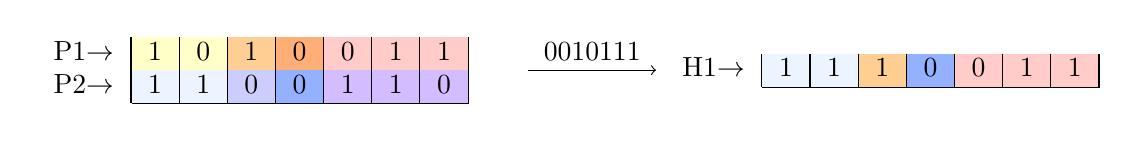
\begin{tikzpicture}
        \node (padres) at (0,0) {\begin{tabular}{l|
            >{\columncolor[HTML]{FFFFC7}}c |
            >{\columncolor[HTML]{FFFFC7}}c |
            >{\columncolor[HTML]{FFCE93}}c |
            >{\columncolor[HTML]{FFAF75}}c |
            >{\columncolor[HTML]{FFCCC9}}c |
            >{\columncolor[HTML]{FFCCC9}}c |
            >{\columncolor[HTML]{FFCCC9}}c |}
            \cline{2-8}
            P1$\rightarrow$ & $1$ & $0$ & $1$ & $0$ & $0$ & $1$ & $1$ \\ \cline{2-8} 
            P2$\rightarrow$ & \cellcolor[HTML]{ECF4FF}$1$ & \cellcolor[HTML]{ECF4FF}$1$ & \cellcolor[HTML]{CBCEFB}$0$ & \cellcolor[HTML]{94B1FF}$0$ & \cellcolor[HTML]{D3BCFF}$1$ & \cellcolor[HTML]{D3BCFF}$1$ & \cellcolor[HTML]{D3BCFF}$0$ \\ \cline{2-8} 
            \end{tabular}};
        \node (hijos) at (8,0) {\begin{tabular}{l|
            >{\columncolor[HTML]{ECF4FF}}c |
            >{\columncolor[HTML]{ECF4FF}}c |
            >{\columncolor[HTML]{FFCE93}}c |
            >{\columncolor[HTML]{94B1FF}}c |
            >{\columncolor[HTML]{FFCCC9}}c |
            >{\columncolor[HTML]{FFCCC9}}c |
            >{\columncolor[HTML]{FFCCC9}}c |}
            \cline{2-8}
            H1$\rightarrow$ & $1$ & $1$ & $1$ & $0$ & $0$ & $1$ & $1$ \\ \cline{2-8} 
            \end{tabular}};
    \draw[-to] (3.5,0) -- (hijos) node[above,midway] {$0010111$};
    \end{tikzpicture}
    \caption{Ejemplo de cruce uniforme con la máscara $0010111$ (cruce equivalente al cruce de 3 puntos con los puntos 2, 3 y 4). En este ejemplo solo se muestra la generación del hijo correspondiente a la máscara, pero se puede generar también el gemelo utilizando la máscara $1101000$.}
    \label{fig:uxcrossover}
\end{figure}

Finalmente el \textbf{cruce no lineal} es necesario para formulaciones de problemas que no permitan los cruces anteriores. El ejemplo más obvio son aquellos problemas cuyas soluciones se encuentren en el espacio de las permutaciones de longitud $l$, $\Pi_l$, como por ejemplo los problemas de rutas que trataremos en este trabajo. Dentro de este tipo de problemas, las soluciones no pueden contener elementos repetidos, por lo que un cruce simple suele generar soluciones no factibles. Para ello utilizaremos cruces no lineales, por ejemplo el PMX o \textbf{cruce parcialmente mapeado}.\\

El PMX es uno de los métodos de cruce no lineal más importante y funciona de la siguiente manera (se puede ver un ejemplo en la Figura \ref{fig:PMX}):
\begin{enumerate}
    \item Se eligen 2 puntos de cruce de manera aleatoria.
    \item Se definen los intercambios a realizar. Para cada valor de $i$ en la región de corte, se definen los intercambios como $P1(i)\leftrightarrow P2(i)$, donde $P2(i)$ define el símbolo que se encuentra en la posición $i$ del cromosoma de padre 2. 
    \item Se intercambian los elementos dentro de cada uno de los padres utilizando las relaciones anteriores (por orden). Es decir, se intercambian los símbolos definidos en las relaciones del paso anterior.
\end{enumerate}

\begin{figure}[t]
    \centering
    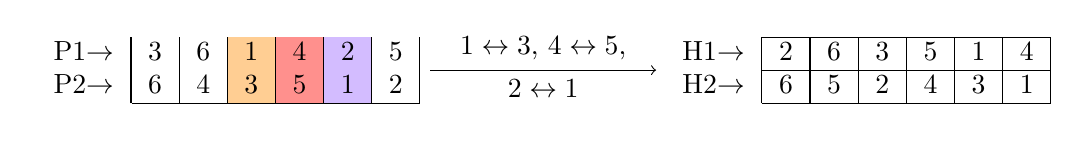
\begin{tikzpicture}
        \node (padres) at (0,0) {\begin{tabular}{l|
        >{\columncolor[HTML]{FFFFFF}}c |
        >{\columncolor[HTML]{FFFFFF}}c |
        >{\columncolor[HTML]{FFCE93}}c |
        >{\columncolor[HTML]{FF908D}}c |
        >{\columncolor[HTML]{D3BCFF}}c |
        >{\columncolor[HTML]{FFFFFF}}c |}
        \cline{2-7}
        P1$\rightarrow$ & $3$ & $6$ & $1$ & $4$ & $2$ & $5$ \\ \cline{2-7} 
        P2$\rightarrow$ & $6$ & $4$ & \cellcolor[HTML]{FFCE93}$3$ & $5$ & $1$ & $2$ \\ \cline{2-7} 
        \end{tabular}};
        \node (hijos) at (8,0) {\begin{tabular}{l|c|c|c|c|c|c|}
            \cline{2-7}
            H1$\rightarrow$ & $2$ & $6$ & $3$ & $5$ & $1$ & $4$ \\ \cline{2-7} 
            H2$\rightarrow$ & $6$ & $5$ & $2$ & $4$ & $3$ & $1$ \\ \cline{2-7} 
            \end{tabular}};
        \draw[-to] (padres) -- (hijos) node[above,midway] {$1\leftrightarrow3$, $4\leftrightarrow5$,} node[below,midway] {$2\leftrightarrow1$};
    \end{tikzpicture}
    \caption{PMX para los puntos de corte 2 y 5.}
    \label{fig:PMX}
\end{figure}

El método de PMX permite realizar cruce con espacios de búsqueda complejos manteniendo la factibilidad de las soluciones. Otra manera de realizar este cruce es mediante el uso de una máscara. Esta máscara se genera igual que en el cruce uniforme pero se aplica de manera diferente. La máscara define qué elementos se mantienen del padre 1 (simbolizado por un 1) y el resto de elementos provienen del segundo padre en el orden en el que estos aparecen.\\

Aunque puede parecer necesario realizar siempre el proceso de cruce, pueden existir situaciones donde este proceso no sea necesario. En la práctica se pueden tomar diversas estrategias, donde se puede usar el proceso de cruce y mutación o solo uno de ellos. En el primer caso, se suelen utilizar dos números $\chi$ y $\mu$, que definen si se realiza cruce y mutación respectivamente. Estos números se utilizan como un umbral, que mediante una distribución uniforme deciden si se realiza o no el proceso de cruce y mutación. En el caso de realizar uno u otro proceso, la probabilidad de elegir cuál utilizar puede ser modificada a lo largo de la ejecución del algoritmo y existen múltiples estrategias para modificar estas probabilidades.
\subsection{Mutación y nueva población}
Finalmente, el último paso para generar la nueva población es el proceso de mutación. La mutación consiste en la modificación aleatoria de uno o varios de los elementos de la cadena $s$. La manera más sencilla para aplicar la mutación es la utilización de una máscara. Estas máscaras son las mismas máscaras que se tratan en la Definición \ref{def:mascara}, sin embargo, en este contexto un 1 significa que se aplica mutación en ese alelo de la cadena. Sin embargo, existen otras variantes para implementar este mecanismo que hacen que cambie significativamente la eficiencia de los algoritmos genéticos.\\

Dentro de estos posibles algoritmos se encuentra la mutación independiente de cada uno de los alelos del cromosoma generado dependiendo de si un número aleatorio se encuentra por debajo de la probabilidad de cruce $\mu$. Sin embargo, aunque efectivo, este método disminuye considerablemente la eficiencia del método de mutación. Una alternativa para mejorar la eficiencia, pero manteniendo la idea, es la utilización de una distribución de Poisson de parámetro $\lambda$, donde el parámetro $\lambda$ define el número medio de mutaciones en cada cromosoma (normalmente se toma $\lambda=1$). Una vez obtenido el número de mutaciones $r$, se eligen aleatoriamente $r$ posiciones en las que realizar la mutación.\\

Hasta ahora solo hemos tratado cuándo hacer la mutación, pero no cómo se hace la mutación. Dado un alfabeto binario, es claro que la mutación consistirá en el cambio de los ceros por unos y viceversa. Sin embargo, en un alfabeto más complejo la mutación es un proceso más complejo y es importante decidir cómo varían los alelos mutados. En los casos en los que no existan restricciones, podemos utilizar una variación aleatoria a otro elemento del alfabeto o una modificación del alelo basándose en una transformación dependiente de una función (se suele utilizar una distribución normal $N(0,\sigma)$). En los casos en los que existen restricciones, podemos utilizar permutaciones de los elementos de la cadena para inducir una mutación \cite{eiben-2003}.\\

La mutación no solo tiene la labor de añadir nueva información a los descendientes que no provenga de los padres, sino que este proceso también sirve para conservar la diversidad de la población y evitar clonaciones (sobre todo cuando el algoritmo se encuentra cerca de un mínimo local).\\

Aunque el proceso original de los algoritmos genéticos solo contenía los pasos tratados anteriormente para la generación de cada nueva generación, en la práctica es importante la adición del concepto del \textbf{elitismo}, que permite que el proceso de búsqueda de óptimos sea más guiado.

\begin{definition}
    El \textit{elitismo} es una estrategia que garantiza que el mejor individuo permanezca para la siguiente generación de la población generando únicamente $M-1$ nuevos individuos. Este proceso puede ser llevado al extremo, sustituyendo solo una fracción $G$ (\textit{brecha generacional}) de la población en cada nueva generación; o simplemente sustituyendo los 2 peores cromosomas (\textit{estrategias incrementales}).
\end{definition}
\subsection{Convergencia teórica}\label{geneticos-conv}
Ahora que hemos tratado el funcionamiento de los algoritmos genéticos en su totalidad podemos preguntarnos si existe una explicación de porqué estos algoritmos son útiles para la optimización de problemas complejos. Aunque realmente no existe una prueba formal que demuestre su funcionamiento, se han debatido distintas ideas y visiones que permiten tratar el buen funcionamiento de estos algoritmos. En este trabajo se resumirá la información tratada en \cite{reeves-2002}.\\

En primer lugar, es importante tratar el motivo por el que la exploración de el espacio de búsqueda $\mathscr{A}^l$ es mejor que la exploración de $\xcal$. La principal idea se basa en la idea de los \textbf{esquemas}.

\begin{definition}
    Un \textit{esquema} es un subconjunto $S\subset \mathscr{A}^l$ donde todos los cromosomas $s\in S$ comparten un conjunto particular de valores definidos. Un esquema puede verse como un alfabeto $S=(\mathscr{A}\cup *)^l$ donde el símbolo $*$ representa cualquier posible valor del alfabeto $\mathscr{A}$. Por ejemplo, el conjunto $S=1\ *\ *\ 0$ representa todos los cromosomas de longitud 4 que tienen un $1$ en la primera posición y un $0$ en la última.
\end{definition}

La primera idea del uso de los esquemas es el paralelismo implícito que existe al utilizar múltiples esquemas. Sin embargo, en la práctica, los esquemas no pueden pueden ser procesados en paralelo ya que no puede estimarse la adecuación simultánea de un conjunto de esquemas. Por ello, los esquemas se pueden utilizar de otra manera, mediante el uso del teorema de los esquemas de Holland. 

\begin{theorem}\label{th:schemas}
    Dado $N(S,t)$ el número de instancias del esquema $S$ en el momento de tiempo $t$, entonces en el siguiente espacio de tiempo (tras la siguiente reproducción), el número esperado de instancias del esquema en la nueva población puede ser acotado por la siguiente expresión:
    \begin{equation*}
        E[N(S,t+1)]\geq\frac{h(S,t)}{\overline{h(t)}}N(S,t)[1- \varepsilon(S,t)],
    \end{equation*}
    donde $h(S,t)$ es la adecuación del esquema $S$, $\overline{h(t)}$ es la media de adecuación de la población y $\varepsilon(S,t)$ define el potencial de que los operadores genéticos destruyan instancias del esquema $S$.
\end{theorem}

Es muy importante que este resultado ofrece una relación estocástica (estamos acotando la esperanza), además de solo ofrecer una acotación para la siguiente generación (si se aplica para más generaciones, no se tiene en cuenta aquellos elementos de la población que dejan de formar parte del esquema $S$). Este teorema es interesante y le da valor al uso de los esquemas para tratar los algoritmos genéticos, sin embargo debido al teorema \textit{No Free Lunch} \cite{nflt}, la idea de tratar un algoritmo genético como un bandido de dos brazos\footnote{Los problemas de bandidos de $n$ brazos son problemas estocásticos en los que se debe elegir uno entre $n$ opciones fijas (o brazos). En estos problemas cada brazo sigue una distribución de probabilidad distinta y deben utilizarse los resultados de anteriores elecciones para decidir qué brazo elegir.} (como múltiples autores hacían originalmente) deja de tener sentido. En esencia, las implicaciones que tiene el teorema \textit{No Free Lunch} para cualquier metaheurística es que, de media, ningún algoritmo es mejor que la búsqueda aleatoria, el encontrar buenas soluciones procede únicamente de la adaptación del algoritmo al problema específico. Esto no implica que el Teorema \ref{th:schemas} sea inútil ya que nos da información de dicha evolución de la población en el siguiente paso de la evolución y existen múltiples investigaciones en este área.\\

Otro de los posibles motivos del funcionamiento de los GA es la idea de la hipótesis de los bloques de construcción. Esta hipótesis indica que la recombinación de los esquemas para formar piezas más grandes es una método para obtener soluciones óptimas. No obstante, existen múltiples pruebas negativas de esta hipótesis.\\

Otros enfoques para el funcionamiento de los algoritmos genéticos son la utilización de la teoría de cadenas de Markov \cite{Vose1995ModelingSG}, la utilización de la mecánica estadística \cite{Shapiro1994ASM} o la relación de los GA con distintos conceptos biológicos. Sin embargo, ninguno de estos métodos han ofrecido conclusiones sobre la convergencia y funcionamiento de los algoritmos. Algunos de los motivos es la falta de la existencia de un algoritmo genético genérico.\\

Múltiples autores han tratado las conexiones que existen entre los algoritmos genéticos y los métodos de búsquedas locales. A partir de estas conexiones se han desarrollado los siguientes algoritmos que trataremos, los algoritmos meméticos, muy útiles en problemas de rutas.
\section{Algoritmos meméticos}
El nombre de algoritmos meméticos es un término genérico utilizado para hacer referencia a un conjunto muy grande de metaheurísticas. Estos métodos tratan de utilizar toda la información posible sobre el problema que se busca resolver. De manera similar al resto de apartados de este capítulo, esta sección se basará en el capítulo 6 del libro \cite{metah-hb}. En primer lugar, se hará una introducción histórica, seguida de una explicación del diseño de los algoritmos meméticos, sus posibles extensiones y los posibles pasos futuros de este tipo de algoritmos

\subsection{Historia}
El nombre de los algoritmos meméticos (MA) viene del término ``meme'', acuñado por Richard Dawkins en \cite{dawkins-1989}. Este término denota el análogo de los genes en el contexto de la evolución cultural. Esta expresión ha sido expandida a lo largo de los años, pero en nuestro caso, el término memético proviene de su definición original. Aquí, que los algoritmos sean denominados ``meméticos'' hace referencia a que en la evolución cultural, los memes no solo transmiten la información sin ser modificada, sino que se produce un proceso de mejora. En los MA, la mejora proviene de la combinación de heurísticas, métodos exactos truncados, operadores de recombinación especializados, \ldots, con el mayor conocimiento del problema posible. La introducción de conocimiento del problema al algoritmo está motivada por resultados teóricos, como puede ser el teorema \textit{No Free Lunch}. Como se trata en la Sección \ref{geneticos-conv}, este teorema implica que para cualquier metaheurística, si no se añade conocimiento del problema, el método de búsqueda equivale a una búsqueda aleatoria.\\

El primer algoritmo memético aparece en el año 1988 y es considerado una hibridación de los algoritmos genéticos tradicionales con el templado simulado \cite{firstma}. Este algoritmo buscaba encontrar los límites de ambas metaheurísticas para la resolución de una versión simplificada del problema del agente viajero (TSP por sus siglas en inglés). En los siguientes años, los autores del anterior algoritmo identificaron otros autores que también buscaban la inclusión de heurísticas en los algoritmos genéticos. De esta manera, el nombre de algoritmos meméticos aparece por primera vez en \cite{memetic-name}, dando lugar a una gran investigación en los últimos años. 
\subsection{Conceptos sobre algoritmos meméticos}
Los conceptos básicos para los algoritmos meméticos se encuentran explicados en la Sección \ref{intro:intro}. Los MA también utilizan los conceptos de los algoritmos genéticos tratados en la Sección \ref{intro:geneticos}, como el cruce y la mutación. En esta sección se mostrará el esquema de aquellos elementos básicos que añaden los algoritmos meméticos y se mostrará su funcionamiento.\\

Como ya se introduce en la historia de los algoritmos meméticos, los MA tienen un esquema similar a un algoritmo genético, sin embargo, el método de generar una nueva población difiere. El esquema principal que sigue cualquier algoritmo memético puede verse en el Algoritmo \ref{alg:memetico}.\\

\begin{algorithm}[!htb]
    \caption{Algoritmo memético}
    \label{alg:memetico}
    \begin{algorithmic}[1]
        \State \textbf{Inicialización:}
        \State Elección de una población inicial
        \State \textbf{Optimización:}
        \While {criterio de terminación no satisfecho}
            \State Generación de una nueva población
            \State Actualización de la población
            \If{la población ha convergido}
            \State Reiniciar la población
            \EndIf
        \EndWhile
    \end{algorithmic}
\end{algorithm}

En este algoritmo, para la elección inicial de la población se pueden utilizar los mismos métodos que se han tratado para la generación de una población inicial en los algoritmos genéticos (véase Sección \ref{intro:sel-inicial}). No obstante, es bastante común que a cada uno de los individuos, escogidos de manera aleatoria, se le aplique una búsqueda local. El criterio de parada es análogo al de los algoritmos genéticos (véase Sección \ref{intro:sel-criterio}). De esta manera, veamos en mayor profundidad el método para la generación de una nueva población, el núcleo de los algoritmos meméticos.\\

El procedimiento de generación de una nueva población puede ser visto como la encadenación de $n_{op}$ pasos. Cada uno de los pasos consiste en la obtención de $l_j$ configuraciones nuevas a partir de $k_j$ configuraciones de entrada utilizando el operador $op_j$. Una restricción que se debe seguir es que $k_1=M$ (donde $M$ es el tamaño total de la población). De esta manera, se obliga a transformar todos los elementos de entrada. El método puede verse representado en el Algoritmo \ref{alg:new-pop}.\\
\begin{algorithm}[!b]
    \caption{Nueva generación}
    \label{alg:new-pop}
    \begin{algorithmic}[1]
        \State \textbf{Inicialización:}
        \State Iniciar la nueva población como la población del paso anterior
        \State \textbf{Optimización:}
        \For {$j\leftarrow1$ \textbf{hasta} $n_{op}$}
            \State Selección de $k_j$ configuraciones de entrada
            \State Aplicar el operador $op_j$ a las $k_j$ configuraciones de entrada
            \State Introducir los $l_j$ elementos generados en la nueva población
        \EndFor
    \end{algorithmic}
\end{algorithm}

Podemos ver que si tomamos $n_{op}=3$ como número de operaciones, donde las operaciones son selección, cruce y mutación, obtendremos un esquema básico de un algoritmo genético. Sin embargo, en los MA se suele utilizar un número de operaciones de $n_{op}=5$, aunque este puede ser superior. El operador que diferencia a los algoritmos meméticos de los genéticos es la búsqueda local. Esta búsqueda local es realizada tras las operaciones de cruce y recombinación y existen diversos métodos para realizarla. Al aplicar una búsqueda local, es importante que el método de mutación no utilice los mismos principios de exploración del vecindario que la búsqueda local (pudiendo hacer inútiles ambos pasos, al revertir la mutación). Una vez generada la nueva población, esta se utilizará para actualizar la población del paso anterior. Existen diversos métodos para actualizar la población, pero generalmente se basan en la proporción de elitismo que se utilice en el método. Otro posible método de actualización es generar de una nueva población de más de $M$ elementos, y tomar los $M$ mejores elementos de esa población.\\

Finalmente, se tiene el paso de reinicio de la población. Este paso tiene lugar en el caso de que la población haya convergido, es decir, que la diversidad de la población sea inferior que un umbral (se dice que la población es degenerada). Para medir la convergencia existen distintos métodos, como puede ser un enfoque bayesiano como puede verse en \cite{Hulin1997AnOS}. Veamos con se realiza el reinicio de la población. En primer lugar, se mantiene un subconjunto de las soluciones de la población degenerada (tan grande como se desee, puede ser solo la mejor solución). Posteriormente, se generan el resto de elementos desde 0, de la misma manera en la que se genera la población inicial.\\

%%%%%%%%% AÑADIR LA PARTE DE "DESIGNING AN EFFECTIVE MEMETIC ALGORITHM" - P64
Este es el esquema fundamental de un algoritmo memético, sin embargo, la resolución de un problema complejo con un MA no es tan sencilla, ya que cada problema deberá utilizar un número y tipo de operaciones específico variable. Esto está respaldado por el teorema \textit{No Free Lunch}. De esta manera, se deberá utilizar el conocimiento existente de los problemas a resolver para obtener un algoritmo memético eficiente, tanto para la parte evolutiva como para la heurística de búsqueda local. 

\subsubsection{Extensiones de los algoritmos meméticos}
Además de los MA ``clásicos'' existen diversas variaciones más sofisticadas que pueden ser requeridas por algunos problemas. Las principales variaciones son:
\begin{itemize}
    \bditem{MA Multiobjetivo:} Los problemas multiobjetivo son muy comunes en la práctica, por lo que deben definirse algoritmos para resolverlos. Este tipo de algoritmos utilizan un orden parcial en la búsqueda que tiene en cuenta las múltiples funciones objetivo. Un posible método para definir el algoritmo es la combinación lineal de las funciones objetivo en una única función.
    \bditem{MA Adaptativo:} En este tipo de algoritmos, la función de generación de una nueva población es modificada a lo largo del proceso de optimización. Generalmente, este tipo de algoritmos tiene un conjunto elevado de posibles operaciones a realizar, y dependiendo del momento de la optimización utiliza unos u otros operadores. Por ejemplo, la optimización puede ser más agresiva al inicio y relajarse a lo largo del tiempo.
    \bditem{MA Completo:} Los algoritmos meméticos completos añaden un proceso de búsqueda exacto a la búsqueda local. De esta manera puede realizarse una exploración más extensa del vecindario, se pueden resolver subproblemas de manera exacta u obtener límites para relajar la búsqueda.
\end{itemize}

\subsubsection{Futuro de los algoritmos meméticos}
El futuro de los algoritmos meméticos parece prometedor. Esto se debe a diversos factores, como la existencia de múltiples implementaciones muy eficientes (aunque en ocasiones muy complejas) con buenos resultados prácticos para varios problemas. Además, en los últimos años, los investigadores creen que será posible establecer límites de complejidad computacional para los algoritmos genéticos. Para obtener estos límites existen distintos enfoques, como puede ser el uso de la teoría de tratabilidad de parámetro fijo\footnote{Este campo trata de clasificar la complejidad computacional en base a un conjunto de parámetros de entrada.}. Por último, debido a la naturaleza de los algoritmos meméticos como algoritmos basados en población, existe un paralelismo implícito que puede ser explotado por los sistemas distribuidos actuales. La paralelización permite la ejecución más veloz de un algoritmo y mediante el uso de lenguajes de programación que permitan este proceso, es posible aumentar la eficiencia de los MA. De esta manera, los algoritmos genéticos son capaces de obtener resultados precisos más rápido que otras metaheurísticas.\\

Una vez vistos los algoritmos que utilizaremos, definamos el problema a resolver: el Problema de Rutas de Camiones y Tráileres Multicompartimento (MC-TTRP por sus siglas en inglés).